% Author Thomas C. Hales
% Copyright 2003, Thomas C. Hales
% AMS-TEX Format
% Revised Oct 4, 2003. Added material on fcc and hcp in Sec. 1

% Reformatted into LaTex. Feb 17, 2004.


%\documentstyle{amsppt}
%\topmatter
%\loadmsbm
%\UseAMSsymbols

%\hoffset=0.75truein
%\voffset=0.5truein


% Intro Historical




The series of papers in this volume gives a proof of the Kepler
conjecture, which asserts that the density of a packing of
congruent spheres in three dimensions is never greater than
$\pi/\sqrt{18}\approx 0.74048\ldots$. This is the oldest problem
in discrete geometry and is an important part of Hilbert's 18th
problem. An example of a packing achieving this density is the
face-centered cubic packing.


\label{sec:intro-review}

\section{The face-centered cubic packing}

A packing of spheres is an arrangement of
nonoverlapping spheres of radius 1 in Euclidean space.
Each sphere is determined by its center, so equivalently it is a collection
of points in Euclidean space separated by distances of at least 2.
The density of a packing is defined as the $\limsup$ of
the densities of the partial packings formed by spheres inside
a ball with fixed center of radius $R$.
(By taking the $\limsup$,
rather than $\liminf$ as the density, we prove the Kepler
conjecture in the strongest possible sense.)
Defined as a limit, the density
is insensitive to changes in the packing in any bounded region.
For example, a finite number of spheres can be removed from the
face-centered cubic packing without affecting its density.

Consequently, it is not possible to hope for any strong uniqueness
results for packings of optimal density.  The uniqueness
established by this work is as strong as can be hoped for. It
shows that certain local structures (centered packings) attached
to the face-centered cubic (fcc) and hexagonal-close packings
(hcp) are the only structures that maximize a local density
function.

Although we do not pursue this point, Conway and Sloane develop
a theory of tight packings that is more restrictive than having the
greatest possible density \cite{CoSl95}.
An open problem is to prove that their
list of tight packings in three dimensions is complete.

The face-centered cubic packing appears in
Diagram~\ref{fig:fcc-pack}.

\begin{figure}[htb]
  \centering
  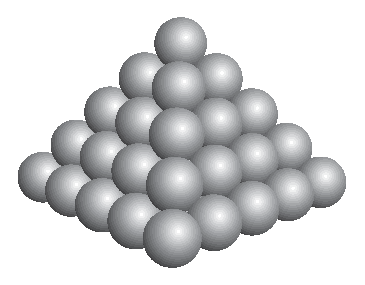
\includegraphics{\ps/fcc_small.eps}
  \caption{The face-centered-cubic packing.}
  \label{fig:fcc-pack}
\end{figure}

The following facts about packings are well-known.  However, there
is a popular and persistent misconception in the popular press
that the face-centered cubic packing is the only packing with
density $\pi/\sqrt{18}$. The comments that follow correct that
misconception.

In the face-centered cubic packing, each ball is tangent to twelve
others.  For each ball in the packing, this arrangement of twelve
tangent balls is the same.  We call it the fcc pattern. In the
hexagonal-close packing, each ball is tangent to twelve others.
For each ball in the packing, the arrangement of twelve tangent
balls is again the same.  We call it the hcp pattern.  The fcc
pattern is different from the hcp pattern.  In the fcc pattern,
there are four different planes through the center of the central
ball that contain the centers of six other balls at the vertices
of a regular hexagon.  In the hcp pattern, there is only one such
plane.  We call the arrangement of balls tangent to a given ball
the {\it local tangent arrangement} of the ball.

There are uncountably many packings of density $\pi/\sqrt{18}$
that have the property that every ball is tangent to twelve others
and such that the tangent arrangement around each ball is either
the fcc pattern or the hcp pattern.

By {\it hexagonal layer}, we mean a translate of the two-dimensional
lattice of points $M$ in the $A_2$ arrangement. That is, $M$ is a
translate of the planar lattice generated by two vectors of length
$2$ and angle $2\pi/3$.  The face-centered cubic packing is an
example of a packing built from hexagonal layers.

If $M$ is a hexagonal layer, a second hexagonal layer $M'$ can be
placed parallel to the first so that each lattice point of $M'$ has
distance $2$ from three different vertices of $M$.  When the second
layer is placed in the manner, it is as close to the first layer as
possible. Fix $M$ and a unit normal to the plane of $M$. The normal
allows us to speak of the second layer $M'$ as being ``above'' or
``below'' the layer $M$. There are two different positions in which
$M'$ can be placed closely above $M$ and two different positions in
which $M'$ can be placed closely below $M$. As we build a packing,
layer by layer, ($M$, $M'$, $M''$, and so forth), there are two
choices at each stage of the close placement of the layer above the
previous layer. Running through different sequences of choices gives
uncountably many packings.  In each of these packings the tangent
arrangement around each ball is that of the twelve spheres in the
face-centered cubic or the twelve spheres in the hexagonal-close
packing.

Let $\Lambda$ be a packing built as a sequence of close-packed
hexagonal layers in this fashion.  If $P$ is any plane parallel to
the hexagonal layers, then there are at most three different
orthogonal projections of the layers $M$ to $P$.  Call these
projections $A$, $B$, $C$.  Each hexagonal layer has a different
projection than the layers immediately above and below it.  In the
fcc packing, the successive layers are $A,B,C,A,B,C,\ldots$.  In
the hcp packing, the successive layers are $A,B,A,B,\ldots$.  If
we represent $A$, $B$, and $C$ as the vertices of a triangle, then
the succession of hexagonal layers can be described by a walk
along the vertices of the triangle. Different walks through the
triangle describe different packings.

% In the face-centered
%cubic packing, every local tangent arrangement of $12$ tangent
%balls is the same.  We call this local tangent arrangement the
%fcc-pattern. Similarly, the local tangent arrangement of the
%hexagonal-close packing will be called the hcp-pattern.  These
%patterns are uniquely determined up to rigid motion.

In fact, the different walks through a triangle give all packings of
infinitely many equal balls in which the tangent arrangement around
every ball is either the fcc pattern of twelve balls or the hcp
pattern of twelve balls.

\bigskip


{

\narrower

\font\ninerm=cmr9 \ninerm

\def\=#1{\accent"16 #1}


We justify the fact that different walks through a triangle give all
such packings. Assume first that a packing $\Lambda$ contains a ball
(centered at $v_0$) in the hcp pattern. The hcp pattern contains a
uniquely determined plane of symmetry. This plane contains $v_0$ and
the centers of six others arranged in a regular hexagonal. If $v$ is
the center of one of the six others in the plane of symmetry, its
local tangent arrangement of twelve balls must include $v_0$ and an
additional four of the twelve balls around $v_0$. These five centers
around $v$ are not a subset of the fcc pattern. They can be uniquely
extended to twelve centers arranged in the hcp pattern. This hcp
pattern has the same plane of symmetry as the hcp pattern around
$v_0$. In this way, as soon as there is a single center with the hcp
pattern, the pattern propagates along the plane of symmetry to
create a hexagonal layer $M$.

Once a packing $\Lambda$ contains a single hexagonal layer, the
condition that each ball be tangent to twelve others forces a
hexagonal layer $M'$ above $M$ and another hexagonal layer below
$M$.  Thus, a single hexagonal layer forces a sequence of
close-packed hexagonal layers in both directions.

We have justified the claim under the hypothesis that $\Lambda$
contains at least one ball with the hcp pattern.

Assume that $\Lambda$ does not contain any balls whose local
tangent arrangement is the hcp pattern.  Then every local tangent
arrangement is the fcc pattern, and $\Lambda$ itself is then the
face-centered cubic packing.  This completes the proof.


}

\section{Early History, Hariot, and Kepler}
\label{sec:early}

The study of the mathematical properties of the face-centered cubic
packing can be traced back to a Sanskrit work composed around 499 CE.
I quote an extensive passage from the commentary that K. Plofker
has made about the formula
for the number of balls in triangular piles\cite{Plo00}:
\medskip

{
\narrower
\font\ninerm=cmr9
\ninerm
\def\=#1{\accent"16 #1}

 The excerpt below is taken
 from a Sanskrit work composed around 499 CE, the \=Aryabha\d t\={\i}ya
 of \=Aryabha\d ta, and the commentary on it written in 629 CE
 by Bh\=askara (I).  The work is a compendium of various rules in
 mathematics and mathematical astronomy, and the results are probably
 not due the \=Aryabha\d ta himself but derived from an earlier source:
 however, this is the oldest source extant for them.  (My translation's
 from the edition by K. S. Shukla, {\it The \=Aryabha\d t\={\i}ya of
 \=Aryabha\d ta with the Commentary of Bh\=askara I and Some\'svara},
 New Delhi: Indian National Science Academy 1976; my inclusions are
 in square brackets. There is a corresponding English translation
 by Shukla and K. V. Sarma, {\it The \=Aryabha\d t\={\i}ya
 of \=Aryabha\d ta}, New Delhi: Indian National Science Academy 1976.
 It might be easier to get hold of the earlier English translation by
 W. E. Clark, {\it The \=Aryabha\d t\={\i}ya of \=Aryabha\d ta},
 Chicago: University of Chicago Press, 1930.)

      Basically, the rule considers the series in arithmetic
 progression
 $
 S_i = 1 + 2 + 3 + \ldots + i
 $
 (for whose sum the formula is known) as the number of objects
 in the $i$th layer of a pile with a total of $n$ layers, and
 specifies the following two equivalent formulas for the ``accumulation
 of the pile'' or $ \sum_{i=1}^n S_i $:

 $$
 \sum_{i=1}^n S_i = \frac{{n(n+1)(n+2)}}{6},
 $$

 $$
 \sum_{i=1}^n S_i = \frac{{(n+1)^3 - (n+1)}}{6}.
 $$

 What he says is this:

 {\it \=Aryabha\d t\={\i}ya}, Ga\d nitap\=ada 21:

 {\narrower
    For a series [lit. ``heap''] with a common difference and first term
 of 1, the product of three [terms successively] increased by 1 from
 the total, or else the cube of [the total] plus 1 diminished by [its]
 root, divided by 6, is the total of the pile [lit. ``solid heap''].
 }

 Bh\=askara's commentary on this verse:

 {\narrower
    [This] heap [or] series is specified as having one for its common
 difference and initial term. This same series with one for its common
 difference and initial term is said [to be] ``heaped up.'' ``The
 product of three [terms successively] increased by one from the total''
 of this so-called heaped-up ``series with one for its common
 difference and initial term'': i.e., the product of three terms, starting
 from the total and increasing by one. Namely, the total, that plus one,
 and [that] plus one again. That [can] be stated [as follows]: the total,
 that plus one, and that total plus two. The product of those three
 divided by 6 is the ``solid heap,'' the accumulation of the series.
 Now another method: The cube of the root equal to that [total] plus
 one is diminished by its root, and divided by 6: thus it follows.
 ``Or else'': [i.e.], the cube of that root plus one, diminished by
 its own root, divided by 6, is the ``solid heap.''
    Example: Series with 5, 8, and 14 respectively for their total layers:
 tell me [their] triangular-shaped piles.
    In order, the totals are 5, 8, 14.
    Procedure: Total 5. This plus one: 6. This plus one again: 7. Product
 of those three: 210. This divided by 6 is the accumulation of the series:
 35.
    [He goes on to give the answers for the second two cases, but you
 doubtless get the picture.]   --  K. Plofker
 }


}



The modern mathematical study of spheres and their close packings can be
traced to T. Hariot.  Hariot's work -- unpublished, unedited,
and largely undated -- shows a preoccupation with sphere packings.
He seems to have first taken an interest in packings at the
prompting of Sir Walter Raleigh.  At the time, Hariot was Raleigh's
mathematical assistant,  and Raleigh gave him the problem of determining
formulas for the number of cannonballs in regularly stacked piles.
In 1591 he prepared a chart of triangular numbers for Raleigh.
Shirley, Hariot's biographer, writes,

{
\narrower
\font\ninerm=cmr9
\ninerm

    Obviously, this is a quick reference chart prepared for Ralegh to give information on the ground space required for the storage of cannon
    balls in connection with the stacking of armaments for his marauding vessels. The chart is ingeniously arranged so that it is possible to
    read directly the number of cannon balls on the ground or in a pyramid pile with triangular, square, or oblong base. All of this Harriot had
    worked out by the laws of mathematical progression (not as Miss Rukeyser suggests by experiment), as the rough calculations
    accompanying the chart make clear. It is interesting to note that on adjacent sheets, Harriot moved, as a mathematician naturally would,
    into the theory of the sums of the squares, and attempted to determine graphically all the possible configurations that discrete particles
    could assume -- a study which led him inevitably to the corpuscular or atomic theory of matter originally deriving from Lucretius and
    Epicurus. \cite[p.242]{Shi83}

}

\smallskip
Hariot connected sphere packings to Pascal's triangle long before
Pascal introduced the triangle. See Diagram~\ref{fig:pascal}.

\begin{figure}[htb]
  \centering
  \includegraphics{\ps/diag21.ps}
  \caption{Hariot's view of Pascal's triangle.}
  \label{fig:pascal}
\end{figure}

Hariot was the first to distinguish between the face-centered
cubic and hexagonal close packings \cite[p.52]{Mas66}.

Kepler became involved in sphere packings through his correspondence
with Hariot in the early years of the 17th century.
Kargon writes, in his history of atomism in England,


{
\narrower
\font\ninerm=cmr9
\ninerm

    Hariot's theory of matter appears to have been virtually that of Democritus, Hero of Alexandria, and, in a large measure, that of Epicurus
    and Lucretius. According to Hariot the universe is composed of atoms with void space interposed. The atoms themselves are eternal and
    continuous. Physical properties result from the magnitude, shape, and motion of these atoms, or corpuscles compounded from them$\ldots$.

    Probably the most interesting application of Hariot's atomic theory was in the field of optics. In a letter to Kepler on 2 December 1606
    Hariot outlined his views. Why, he asked, when a light ray falls upon the surface of a transparent medium, is it partially reflected and
    partially refracted? Since by the principle of uniformity, a single point cannot both reflect and transmit light, the answer must lie in the
    supposition that the ray is resisted by some points and not others.

    ``A dense diaphanous body, therefore, which to the sense appears to be continuous in all parts, is not actually continuous. But it has
    corporeal parts which resist the rays, and incorporeal parts vacua which the rays penetrate$\ldots$''

    It was here that Hariot advised Kepler to abstract himself mathematically into an atom in order to enter `Nature's house'. In his reply of 2
    August 1607, Kepler declined to follow Harriot, ad atomos et vacua. Kepler preferred to think of the reflection-refraction problem in terms
    of the union of two opposing qualities --
    transparence and opacity. Hariot was surprised. ``If those assumptions and reasons satisfy you, I
    am amazed.'' \cite[p.26]{Kar66}

}

\smallskip
Despite Kepler's initial reluctance to adopt an atomic theory, he
was eventually swayed, and in 1611 he published an essay that
explores the consequences of a theory of matter composed of small
spherical particles.  Kepler's essay was the ``first recorded step
towards a mathematical theory of the genesis of inorganic or
organic form'' \cite[p.v]{Why66}.

Kepler's essay describes
the face-centered cubic packing and asserts that ``the packing will
be the tightest possible, so that in no other arrangement  could more
pellets be stuffed into the same container.''  This assertion has
come to be known as the Kepler conjecture.   The purpose of this
collection of papers is to give a proof of this conjecture.

\section{History}
\label{sec:history}

The next episode in the history of this problem is a debate between
Isaac Newton and David Gregory.  Newton and Gregory discussed the
question of how many spheres of equal radius can be arranged to
touch a given sphere.  This is the three-dimensional analogue of the
simple fact that in two dimensions six pennies, but no more, can be
arranged to touch a central penny.  This is the kissing-number
problem in $n$-dimensions. In three dimensions, Newton said that the
maximum was twelve spheres, but Gregory claimed that thirteen might
be possible.

Newton was correct.
In the 19th century, the first papers claiming a proof of the
kissing-number problem appeared
in \cite{Ben74}, \cite{Gun75}, \cite{Hop74}.
Although some writers cite these papers
as a proof, they are hardly rigorous by today's standards.
Another incorrect
proof appears in \cite{Boe52}.
  The first proper proof was obtained
by B. L. van der Waerden and Sch\"utte in 1953 \cite{Sch53}.
An elementary proof appears in Leech \cite{Lee56}.
The influence of van der Waerden, Sch\"utte, and Leech upon the
papers in this collection is readily apparent.  Although the
connection between the Newton-Gregory problem and Kepler's problem
is not obvious, L. Fejes T\'oth in 1953, in the first
work describing a strategy to prove the Kepler conjecture, made
a quantitative version of the Gregory-Newton problem the first step
\cite{Fej53}.


The two-dimensional analogue of the Kepler conjecture is to show
that the honeycomb packing in two dimensions gives the highest
density.  This result was established in 1892 by Thue, with a second
proof appearing in 1910 (\cite{Thu92}, \cite{Thu10}). G. Szpiro's
book on the Kepler conjecture calls Thue's proofs into question
(\cite{Szp02}).  C. Siegel said that Thue's original proof is
``reasonable, but full of holes'' (\cite{Szp02}). A number of other
proofs have appeared since then. Three are particularly notable.
Rogers's proof generalizes to give a bound on the density of
packings in any dimension \cite{Rog58}. A proof by L. Fejes T\'oth
extends to give bounds on the density of packings of convex disks
\cite{Fej50}. A third proof, also by L. Fejes T\'oth, extends to
non-Euclidean geometries \cite{Fej53}. Another early proof appears
in \cite{SeM44}.

In 1900, Hilbert made the Kepler conjecture part of his 18th
problem \cite{hilbert}. Milnor, in his review of Hilbert's 18th
problem, breaks the problem into three parts \cite{Mil76}.

{
\narrower
\font\ninerm=cmr9
\ninerm

1.  Is there in $n$-dimensional Euclidean Space $\ldots$ only a finite
number of essentially different kinds of groups of motions with a
[compact] fundamental region?

2.  Whether polyhedra also exist which do not appear as fundamental
    regions of groups of motions, by means of which nevertheless
    by a suitable juxtaposition of congruent copies a complete filling
    up of all [Euclidean] space is possible?

3.  How can one arrange most densely in space an infinite number
    of equal solids of given form, e.g. spheres with given radii $\ldots$,
    that is, how can one so fit them together that the ratio of the
    filled to the unfilled space may be as great as possible?

}

\smallskip
Writing of the third part, Milnor states,

{
\narrower
\font\ninerm=cmr9
\ninerm

For $2$-dimensional disks this problem has been solved by Thue and
Fejes T\'oth, who showed that the expected hexagonal (or honeycomb)
packing of circular disks in the plane is the densest possible.
However, the corresponding problem in $3$ dimensions remains
unsolved. This is a scandalous situation since the (presumably)
correct answer has been known since the time of Gauss. (Compare
Hilbert and Cohn-Vossen.)  All that is missing is a proof.

}

\section{The Literature}

Past progress toward the Kepler conjecture can be arranged into
four categories:
\begin{itemize}
    \item bounds on the density,
    \item descriptions of classes of packings for
which the bound of $\pi/\sqrt{18}$ is known,
    \item convex bodies other
than spheres for which the packing density can be determined
precisely,
    \item strategies of proof.
\end{itemize}

%\subhead 4.1. Bounds\endsubhead
\subsection{Bounds}

Various upper bounds have been established on the density of
packings.
\smallskip

{\obeylines

 \ 0.884\ \ (Blichfeldt) \cite{Bli19},
 \ 0.835\ \ (Blichfeldt) \cite{Bli29},
 \ 0.828\ \ (Rankin) \cite{Ran47},
 \ 0.7797\ (Rogers) \cite{Rog58},
 \ 0.77844 (Lindsey) \cite{Lin86},
 \ 0.77836 (Muder)\cite{Mud88},
 \ 0.7731\ (Muder) \cite{Mud93}.

}

\smallskip
Rogers's is a particularly natural bound.
  As the dates indicate, it remained the best available
bound for many years.  His monotonicity lemma and his
decomposition of Voronoi cells into simplices have become important
elements in the proof of the Kepler conjecture.
We give a new proof of Rogers's bound
in ``Sphere Packings III.''  A function $\tau$,
used throughout this
collection, measures the departure of various objects from
Rogers's bound.

Muder's bounds, although they appear to be rather small
improvements of Rogers's bound, are the first to make use of the
full Voronoi cell in the determination of densities. As such, they
mark a transition to a greater level of sophistication and
difficulty.  Muder's influence on the work in this collection is
also apparent.

A sphere packing admits a Voronoi decomposition: around
every sphere take the convex region consisting of points closer to that sphere
center than to any other sphere center.   L. Fejes T\'oth's
dodecahedral
conjecture asserts that the Voronoi cell of smallest volume is
a regular dodecahedron with inradius 1 \cite{Fej42}.
The dodecahedral conjecture implies a bound of 0.755 on sphere
packings.  L. Fejes T\'oth actually gave a complete proof except
for one estimate. A footnote in his paper documents the gap, ``In the
proof, we have relied to some extent solely on intuitive
observation [Anschauung].''
 As L. Fejes T\'oth pointed out, that estimate is extraordinarily
difficult, and the dodecahedral conjecture has resisted all efforts
until now \cite{McL98}.

The missing estimate in L. Fejes T\'oth's paper is an explicit form
of the Newton-Gregory problem.  What is needed is an explicit bound
on how close the 13th sphere can come to touching the central
sphere.  Or more generally, minimize the sum of the distances
of the 13 spheres from the central sphere.
No satisfactory bounds are known.  Boerdijk has a conjecture for the arrangement
that minimizes the average distance of the 13 spheres from the
central sphere.   Van der Waerden
has a conjecture for the closest arrangement of 13 spheres in which
all spheres have the same distance from the central sphere.
Bezdek has shown that the dodecahedral conjecture would follow from
weaker bounds than those originally proposed by L. Fejes T\'oth
\cite{Bez97}.

A proof of the dodecahedral conjecture has traditionally been
viewed as the first step toward a proof of the Kepler conjecture,
and if little progress has been made until now toward a complete
solution of the Kepler conjecture, the difficulty of the dodecahedral
conjecture is certainly responsible to a large degree.

\subsection{Classes of packings}

If the infinite dimensional space of all packings is too unwieldy,
we can ask if it is possible to establish the bound $\pi/\sqrt{18}$
for packings with special structures.

If we restrict the problem
to packings whose sphere centers are the points of a lattice, the
 packings are described by a finite number of parameters, and the
problem becomes much more accessible.  Lagrange proved that the
densest lattice packing in two dimensions is the familiar honeycomb
arrangement \cite{Lag73}. Gauss proved that the densest lattice
packing in three dimensions is the face-centered cubic \cite{Gau31}.
In dimensions 4--8, the optimal lattices are described by their root
systems, $A_2$, $A_3$, $D_4$, $D_5$, $E_6$, $E_7$, and $E_8$. A.
Korkine and G. Zolotareff showed that $D_4$ and $D_5$ are the
densest lattice packings in dimensions 4 and 5 (\cite{KoZ73},
\cite{KoZ77}). Blichfeldt determined the densest lattice packings in
dimensions 6--8 \cite{Bli35}. Cohn and Kumar solved the problem in
dimension 24 \cite{CoKu}.  With the exception of dimension $24$,
beyond dimension $8$, there are no proofs of optimality, and yet
there are many excellent candidates for the densest lattice
packings.  For a proof of the existence of optimal lattices, see
\cite{Oes90}.


Although lattice packings are of particular interest because they
relate to so many different branches of mathematics, Rogers has
conjectured that in sufficiently high dimensions, the densest
packings are not lattice packings \cite{Rog64}.   In fact, the
densest known packings in various dimensions are not lattice
packings.  The third edition of \cite{CS} gives several examples
of nonlattice packings that are denser than any known lattice
packings (dimensions 10, 11, 13, 18, 20, 22). The densest packings
of typical convex sets in the plane, in the sense of Baire
categories, are not lattice packings \cite{Fej95}.

Gauss's theorem on lattice densities has been generalized by
A. Bezdek, W. Kuperberg, and E. Makai, Jr. \cite{BKM91}.
They showed that packings of parallel
strings of spheres never have density greater than $\pi/\sqrt{18}$.

\subsection{Other convex bodies}

If the optimal sphere packings are too difficult to determine,
we might ask whether
the problem can be solved for other convex bodies.
To avoid trivialities, we restrict our attention to convex bodies
whose packing density is strictly less than 1.

  The first convex body in Euclidean 3-space that does not tile
for which the packing density was explicitly determined is
an infinite cylinder \cite{Bez90}.
Here A. Bezdek and W. Kuperberg prove
that the
optimal density is obtained by arranging the cylinders in
parallel columns in the honeycomb arrangement.

In 1993, J. Pach exposed the humbling depth of our ignorance when he issued
the challenge to determine the packing density for some bounded convex
body that does not tile space \cite{MP93}.
(Pach's question is more revealing than anything I can write on
the subject of discrete geometry.)
 This question was answered by
A. Bezdek \cite{Bez94}, who determined the packing density of a rhombic
dodecahedron that has one corner clipped so that it no longer tiles.
The packing density equals the ratio of the
volume of the clipped
rhombic dodecahedron to the volume of the unclipped rhombic dodecahedron.

\subsection{Strategies of proof}

In 1953, L. Fejes T\'oth proposed a program to prove the
Kepler conjecture \cite{Fej53}.
A single Voronoi cell cannot lead to a bound better
than the dodecahedral conjecture.   L. Fejes T\'oth considered
weighted averages of the volumes of collections of Voronoi cells.
 These weighted
averages involve up to 13 Voronoi cells.  He showed that if a particular
weighted average of volumes is greater than the volume of the
rhombic dodecahedron, then the Kepler conjecture follows.
The Kepler conjecture is an optimization problem in an infinite
number of variables.  L. Fejes T\'oth's weighted-average argument
was the first indication that it might be possible to reduce
the Kepler conjecture to a problem in a finite number of variables.
Needless to say, calculations involving the weighted averages of the
volumes of
several Voronoi cells will be significantly more difficult than those
involved in establishing the dodecahedral conjecture.

To justify his approach, which limits the number of Voronoi cells
to 13, Fejes T\'oth needs a preliminary estimate of how close
a 13th sphere can come to a central sphere.  It is at this point
in his formulation of the Kepler conjecture that an explicit
version of the Newton-Gregory problem is required.  How
close can 13 spheres come to a central sphere, as measured by
the sum of their distances from the central sphere?

%Strictly speaking, neither L. Fejes T\'oth's program nor my own program
%educes the Kepler
%conjecture to a finite number of variables, because if
%it turned out that one of
%the optimization problems in finitely many
%variables had an unexpected global maximum, the program would
%fail, but the Kepler conjecture would remain intact.
%In fact, the failure of a program has
%no implications for the Kepler conjecture.  The proof that the
%Kepler conjecture reduces to a finite number of variables comes only as
%corollary to the full proof of the Kepler conjecture.

L. Fejes T\'oth made another significant suggestion in \cite{Fej64}.
He was the first to suggest the use of computers in the Kepler conjecture.
After describing his program, he writes,

{
\narrower
\font\ninerm=cmr9
\ninerm

Thus it seems that the problem can be reduced to the determination
of the minimum of a function of a finite number of variables,
providing a programme realizable in principle.  In view of the
intricacy of this function we are far from attempting to
determine the exact minimum.  But, mindful of the rapid development
of our computers, it is imaginable that the minimum may
be approximated with great exactitude.

}

\smallskip
The most widely publicized attempt to prove the Kepler conjecture
was that of Wu-Yi Hsiang \cite{Hsi93}.  (See also \cite{Hsi93a},
\cite{Hsi93b}, \cite{Hsi02}.)  Hsiang's approach can be viewed as
a continuation and extension of L. Fejes T\'oth's program.
Hsiang's paper contains major gaps and errors \cite{CoHMS94}.
  The mathematical arguments against his argument appear
in my
debate with him in the {\it Mathematical Intelligencer}
(\cite{Hal94}, \cite{Hsi95}).
There are now many published sources that agree with the central
claims of \cite{Hal94} against Hsiang.
Conway and Sloane report that the paper ``contains serious flaws.''
G. Fejes T\'oth feels that ``the greater part of the work has yet
to be done'' \cite{Fej95}.   K. Bezdek concluded,
after an extensive study of Hsiang's work, ``his work is far from being
complete and correct in all details'' \cite{Bez97}.
 D. Muder writes, ``the
community has reached a consensus on it: no one buys it'' \cite{Mud97}.


\chapter{Overview of the proof}

\section{Experiments with other Decompositions}
\label{sec:experiment}

The following two sections (added Jan 2003)  describe some of the
motivation behind the partitions of space that have been used in the
proof of the Kepler conjecture.  This discussion includes various
ideas that were tried, found wanting, and discarded. However, this
discussion provides motivation for some of the choices that appear
in the proof of the Kepler conjecture.

Let $S$ be a regular tetrahedron of side length $2$.  If we place a
unit ball at each of the four vertices, the fraction of the
tetrahedral solid occupied by the part of the four balls within the
tetrahedron is $\dtet\approx 0.7797$. Let $O$ be a regular
octahedron of side length $2$.  If we place a unit ball at each of
the four vertices, the fraction of the octahedral solid occupied by
the four balls is $\doct\approx 0.72$. The face-centered cubic
packing can be obtained by packing eight regular tetrahedra and six
regular octahedra around each vertex. The density $\pi/\sqrt{18}$ of
this packing is a weighted average of $\dtet$ and $\doct$:
    $$\frac\pi{\sqrt{18}} = \frac13\dtet + \frac23\doct.$$

My early conception (around 1989) was that for every packing of
congruent balls, there should be a corresponding partition of space
into regions of high density and regions of low density. Regions of
high density should be defined as regions having density between
$\doct$ and $\dtet$, and regions of low density should be defined as
those regions of density at most $\doct$.  It was my intention to
prove that all regions of high density had to be confined to a set
of nonoverlapping tetrahedra whose vertices are centers of the balls
in the packing.

Thus, the question naturally arises of how much a regular
tetrahedron of edge length $2$ can be deformed before its density
drops below that of a regular octahedron $\doct$.  The following
graph (Figure~\ref{fig:t51}) shows the density of a tetrahedron with
five edges of length $2$ and a sixth edge of length $x$.
Numerically, we see that the density drops below $\doct$, when
$x=x_0\approx 2.504$. To achieve the design goal of confining
regions of high density to tetrahedra, we want a tetrahedron of edge
lengths $2,2,2,2,2,x$, for $x\le x_0$, to be counted as a region of
high density. Rounding upward, this example led to the cutoff
parameter of $2.51$ that distinguishes the tetrahedra (in the high
density region) from the rest of space. This is the origin of the
constant $2.51$ that appears in the proof.


\begin{figure}[htb]
  \centering
  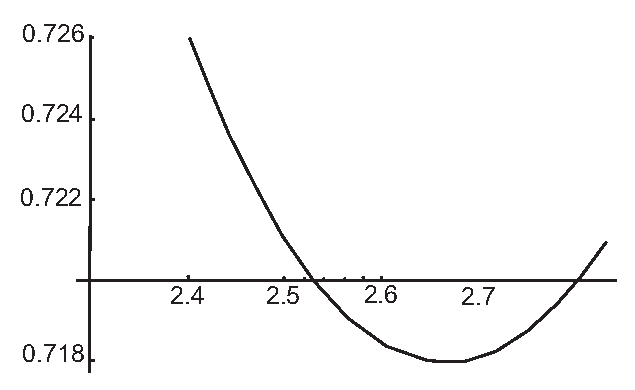
\includegraphics{\ps/t51.eps}
  \caption{The origin of the constant $2.51$.}
  \label{fig:t51}
\end{figure}

Since the tetrahedra are chosen to have vertices at the centers of
the balls in the packing, it was quite natural to base the
decomposition of space on the Delaunay decomposition. According to
this early conception, space was to be partitioned into Delaunay
simplices.  A Delaunay simplex whose edge lengths are at most
$2.51$ is called a quasi-regular tetrahedron.  These were the
regions of presumably high density.  According to the strategy in
those early days, all other Delaunay simplices were to be shown to
belong to regions of density at most $\doct$.

The following problem occupied my attention for a long period.


\smallskip\noindent
{\bf Problem} Fix a saturated packing. Let $X(oct)$ be the part of
space of a saturated packing that is occupied by the Delaunay
simplices having at least one edge of length at least $2.51$.  Let
$X(tet)$ be the union of the complementary set of Delaunay
simplices.  Is it always true that the density of $X(oct)$ is at
most $\doct$?

Early on, I viewed the positive resolution of this problem as
crucial to the solution of the Kepler conjecture.  Eventually,
when I divided the proof of the Kepler conjecture into a five step
program, a variant of this problem became the second step of the
program. See \cite{part2}.

To give an indication of the complexity of this problem, consider
the simplex with edge lengths $(2,2,2,2,\ell,\ell)$, where $\ell =
\sqrt{2 (3 + \sqrt6)}\approx 3.301$.  Assume that the two longer
edges meet at a vertex.  This simplex can appear as the Delaunay
simplex in a saturated packing.  Its density is about $0.78469$.
This constant is not only greater than $\doct$; it is even greater
than $\dtet$, so that the problem is completely misguided at the
level of individual Delaunay simplices in $X(oct)$.  It is only in
when the union of Delaunay simplices is considered that we can
hope for an affirmative answer to the problem.

By the summer of 1994, I had lost hope of finding a partition of
the set $X(oct)$ into small clusters of Delaunay simplices with
the property that each cluster had density at most $\doct$.
Progress had ground to a halt.   The key insight came in the fall
of 1994 (on Nov 12, 1994 to be precise). On that day, I introduced
a hybrid decomposition that relied on the Delaunay simplices in
the regions $X(tet)$ formed by quasi-regular tetrahedra, but that
switched to the Voronoi decomposition in certain regions of
$X(oct)$. By April 1995, I had reformulated the problem, worked
out a proof of the problem \cite{part2} in its new form, and
submitted it for publication. I submitted a revised version of
\cite{part1} that same month.  The revision mentions the new
strategy: ``The rough idea is to let the score of a simplex in a
cluster be the compression $\Gamma(S)$ [a function based on the
Delaunay decomposition] if the circumradius of every face of $S$
small, and otherwise to let the score be defined by Voronoi cells
(in a way that generalizes the definition for quasi-regular
tetrahedra).'' See \cite[p.6]{part1}.

The situation is somewhat more complicated than the previous
paragraph suggests. Consider a Delaunay simplex $S$ with edge
lengths $(2,2,2,2,2,2.52)$. Such a simplex belongs to the region
$X(oct)$. However, if we break it into four pieces according to
the Voronoi decomposition, the density of the two of the pieces is
about $0.696<\doct$ and the density of the other two is about
$0.7368>\doct$. It is desirable not to have any separate regions
in $X(oct)$ of density greater than $\doct$.  Hence it is
preferable to keep the four Voronoi regions in $S$ together as a
single Delaunay simplex.  A second reason to keep $S$ together is
that the proof of the local optimality of the face-centered cubic
packing and hexagonal close packing seems to require it.  A third
reason was to treat pentahedral prisms.  (This is a thorny class
of counterexamples to a pure Delaunay simplex approach to the
proof of the Kepler conjecture.  See \cite{spp}, \cite{remarks},
and \cite{Fer97}.)  For these reasons, we identify a class of
Delaunay simplices in $X(oct)$ (such as $S$) that are to be
treated according to a special set of rules. They are called {\it
quarters}.  As the name suggests, they often occur as the four
simplices comprising an octahedron that has been ``quartered.''

One of the great advantages of a hybrid approach is that there is
a tremendous amount of flexibility in the choice of the details of
the decomposition.  The details of the decomposition continued to
evolve during 1995 and 1996.  Finally, during a stay in Budapest
following the Second European Congress in 1996, I abandoned all
vestiges of the Delaunay decomposition, and adopted definitions of
quasi-regular tetrahedra and quarters that rely only on the metric
properties of the simplices (as opposed to the Delaunay criterion
based on the position of other sphere centers in relation to the
circumscribing sphere of the simplex).  This decomposition of
space is essentially what is used in the final proof.

The hybrid construction depends on certain choices of functions
(satisfying a rather mild set of constraints).  To solve the
Kepler conjecture appropriate functions had to be selected, and an
optimization problem based on those functions had to be solved.
This function is called {\it the score}.  Samuel Ferguson and I
realized that every time we encountered difficulties in solving
the minimization problem, we could adjust the scoring function
$\sigma$ to skirt the difficulty.  The function $\sigma$ became
more complicated, but with each change we cut months -- or even
years -- from our work.  This incessant fiddling was unpopular
with my colleagues.  Every time I presented my work in progress at
a conference, I was minimizing a different function.  Even worse,
the function was mildly incompatible with what I did in earlier
papers \cite{part1} \cite{part2}, and this required going back and
patching the earlier papers.

The definition of the scoring function $\sigma$ did not become
fixed until it came time for Ferguson to defend his thesis, and we
finally felt obligated to stop tampering with it.  The final
version of the scoring function $\sigma$ is rather complicated.
The reasons for the precise form of $\sigma$ cannot be described
without a long and detailed description of dozens of sphere
clusters that were studied in great detail during the design of
this function. However, a few general design principles can be
mentioned.  These comments assume a certain familiarity with the
design of the proof.


(1) Simplices (with vertices at the centers of the balls in the
packing) should be used whenever careful estimates of the density
are required.  Voronoi cells should be used whenever crude
estimates suffice.  For Voronoi cells, it is clear what the
scoring function should be $\vor(R)$ (and its truncated versions
$\vor_0(R)$, and so forth).


(2) The definition of the scoring function for quasi-regular
tetrahedra was fixed by \cite{part1} and this definition had to
remain fixed to avoid rewriting that long paper.

Because of these first two points, most of the design effort for
the function $\sigma$ was focused on quarters.

(3)  The decision to make the scoring for a quarter change when
the circumradius of a face reaches $\sqrt2$ is to make the proof
of the local optimality of the fcc and hcp packings run smoothly.
From \cite{part2}, we see that the cutoff value $\sqrt2$ is
important for the success of that proof.  The cutoff $\sqrt2$ is
also important for the proof that standard regions (other than
quasi-regular tetrahedra) score at most $0\,\pt$.

(4) The purpose of adding terms to the scoring function $\sigma$
that depend on the truncated Voronoi function $\vor_0$ is to make
interval arithmetic comparisons between $\sigma$ and $\vor_0$
easier to carry out.  This is useful in arguments about ``erasing
upright quarters.''

\section{Contents of the Papers}

In \cite{part1}, a five-step program was described to prove the
Kepler conjecture.  It was planned that there would be five
papers, each proving one step in the program.  The papers
\cite{part1} and \cite{part2} carry out the first two steps in the
program. Because of the changes in the scoring function, it was
necessary to issue a short paper \cite{Form} mid-stream whose
purpose was to give some adjustments to the five-step program.
This paper adjusts the definitions from \cite{part1} and checks
that none of the results from \cite{part1} and \cite{part2} are
affected in an essential way by these changes. Following this, the
papers \cite{Hal98B} and \cite{Fer97} appeared in preprint form,
completing the third and fifth steps of the program. The fourth
step turned out to be particularly difficult. It occupies two
separate papers \cite{Hal98C} and \cite{Hal98D}.

The original series of papers suffers from the defect of being
written over a span of several years.  Some shifts in the
conceptual framework of the research are evident.   Based on
comments from referees, a revision of these papers was prepared in
2002. The revisions were small, except for the paper
\cite{Hal98D}, which was completely rewritten. The structure of
the proof remains the same, but it adds a substantial amount of
introductory material that lessens the dependence on \cite{part1}
and \cite{part2}.

The papers were reorganized again in 2003.  The series of papers
is no longer organized along the original five steps with a
mid-stream correction.  Instead, the proof is now arranged
according to the logical development of the subject matter.  Only
minor modifications have been made to the original proof.  (The
earlier versions are still available from \cite{arXiv}.)  In the
2003 revision, the exposition of the proof is entirely independent
of the earlier papers \cite{part1} and \cite{part2}.

An introduction to the ideas of the proof can be found in
\cite{CH}. An introduction to the algorithms can be found at
\cite{algorithm}. Speculation on a second-generation design of a
proof can be found in \cite{algorithm} and \cite{arbeitstagung}.


\section{Complexity}

Why is this a difficult problem?  There are many ways to answer this
question.

This is an optimization problem in an infinite number of
variables.  In many respects, the central problem has been to
formulate a good finite dimensional approximation to the density
of a packing.  Beyond this, there remains an extremely difficult
problem in global optimization, involving nearly 150 variables.
We recall that even very simple classes of nonlinear optimization
problems, such as quadratic optimization problems, are NP-hard
\cite{HoPT95}.  A general highly nonlinear program of this size is
regarded by most researchers as hopeless (at least as far as
rigorous methods are concerned).

There is a considerable literature on many closely related nonlinear
optimization problems (the Tammes problem, circle packings, covering
problems, the Lennard-Jones potential, Coulombic energy minimization
of point particles, and so forth). Many of our expectations about
nonlattice packings are formed by the extensive experimental data
that have been published on these problems. The literature leads one
to expect a rich abundance of critical points, and yet it leaves one
with a certain skepticism about the possibility of establishing
general results rigorously.

The extensive survey of circle packings
in \cite{Mel97} gives a broad overview of the progress and limits
of the subject.
Problems involving a few circles can be
trivial to solve.
Problems involving several circles in the plane can be solved with
sufficient ingenuity.
With the aid of computers, various  problems involving
a few more circles can be
treated by rigorous methods.
Beyond that, numerical methods
give approximations but no rigorous solutions.
Melissen's account of
the 20-year quest for the best separated arrangement of 10
points in a unit square is particularly revealing of the complexities
of the subject.

Kepler's problem has a particularly rich collection of (numerical)
local maxima that come uncomfortably close to the global maximum
\cite{spp}. These local maxima explain in part why a large number
(around 5000) of planar maps are generated as part of the proof of
the conjecture.  Each planar map leads to a separate nonlinear
optimization problem.



\section{Computers}

As this project has progressed, the computer has replaced conventional
mathematical arguments more and more, until now
 nearly every aspect of the proof relies on
computer verifications.  Many assertions in these papers
 are results of computer calculations.
To make the proof of Kepler's conjecture more accessible, I have
posted extensive resources \cite{arXiv}.

Computers are used in various significant ways.  They will be
mentioned briefly here, and then developed more thoroughly elsewhere
in the collection, especially in the final paper.

1. {\it  Proof of inequalities by interval arithmetic}.  ``Sphere Packings
I'' describes a method of proving various inequalities in a small number
of variables by computer by interval arithmetic.

2.  {\it Combinatorics}.  A computer program classifies all of the planar maps
that are relevant to the Kepler conjecture.

3. {\it  Linear programming bounds}.  Many of the nonlinear optimization
    problems for the scores of centered packings are replaced by linear
    problems that dominate the original score.  They are solved
    by linear programming methods by computer.  A typical problem has
    between 100 and 200 variables and 1000 and 2000 constraints.  Nearly
    100000
    such problems enter into the proof.

4. {\it Branch and bound methods}.  When linear programming methods do not
    give sufficiently good bounds, they have been combined with branch
    and bound methods from global optimization.

5.  {\it Numerical optimization}.  The exploration of the problem
    has been substantially
    aided by nonlinear optimization and symbolic math packages.

6. {\it Organization of output}.
    The organization of the few gigabytes of code and data that
    enter into the proof is in itself a nontrivial undertaking.
